\begin{abstract}
MARA is a local-first workbench for document question answering over mixed technical and academic collections. It extends a basic local QA framework, inherited from Kotaemon, with a route-aware controller, shared Web and CLI workflows, multimodal evidence routes, citation and trace observability, and a benchmark harness for route-level diagnosis. The main technical feature is a Self-RAG-inspired controller implemented as explicit program decisions rather than as a trained reflection-token model. Given a question and selected sources, the controller inspects text, visual, element, and graph evidence availability; starts from fixed, planner-supplied, or heuristic route decisions; applies heuristic route-scoring proxies when probe evidence is available; selects among text RAG, page-image/VLM, hybrid, guarded retrieval, graph, direct, and abstention behaviours; and returns answer, citation, evidence, workflow-cost, and verification traces. A full-system benchmark over 41 completed artifact sets and 3,540 prediction records shows that MARA's controller behaviour is measurable across text-heavy, citation-grounded, and multimodal QA settings. The paper presents the approach, experiments and results, demonstration use case, related work, and the engineering limitations that remain before broader deployment.
\end{abstract}

\section{Introduction}

Document question answering systems are useful only when users can see why an answer was produced. A single fixed retrieval-augmented generation (RAG) path can answer many text-heavy questions, but practical document work involves tables, slide images, page layouts, cross-document summaries, incomplete evidence, and cases where the safest output is to abstain. These cases are common in academic and technical collections: a user may ask for a numerical value in a report, an evidence-backed answer in a paper, or a visual detail on a slide. In each case, the system should choose an appropriate route, expose the evidence it used, and avoid unsupported claims.

MARA, short for Multimodal Agentic Retrieval and Answering, is a local-first multimodal document QA workbench built for this setting. It is not a new foundation model. Instead, it is a demonstrable system that extends a Kotaemon-style local QA baseline \citep{kotaemon}. The inherited baseline already supports file upload, model configuration, and a standard document QA flow. MARA focuses on the controller-centred extension: route-aware retrieval and answering, evidence checking, citation and trace observability, multimodal routes, shared Web/CLI workflows, and benchmark-backed evaluation of these behaviours.

The distinguishing idea is a Self-RAG-inspired controller. Self-RAG treats retrieval and critique as explicit decisions \citep{asai2023selfrag}; MARA adapts this idea at the system level. Rather than training a model with reflection tokens, MARA records ordinary program decisions: whether to retrieve, which route to use, whether evidence is adequate, whether a higher-cost route is justified, whether to switch routes, and whether to abstain. This design keeps the system feasible as a local prototype while preserving the core research question: can route-aware control make a document QA workbench more transparent and reliable than a fixed RAG pipeline?

The demo target is a system paper rather than a leaderboard paper. The user-facing workflow shows a corpus, a page/evidence preview, a QA panel, citations, controller trace, and verification metadata. The non-UI workflow exposes the same runtime through the \texttt{MARA docqa} CLI. Optional Codex and Claude Code skill wrappers install documented command families for external coding assistants, but the system boundary remains the local MARA runtime. The benchmark workflow evaluates route behaviour from manifests, predictions, route metrics, and synthesis reports.

This paper makes three contributions:
\begin{itemize}
    \item A local-first multimodal document QA workbench exposing the same QA workflow through Web UI, local CLI, and optional agent-platform wrappers.
    \item A traceable Self-RAG-inspired controller that selects among text, visual, hybrid, CRAG-guarded, graph, direct, and abstention behaviours using route probes, heuristic route-scoring proxies, workflow-cost annotations, evidence checks, route switching, and verification traces.
    \item A benchmark-backed demonstration using a full-system benchmark to compare routes across QASPER, ALCE-ASQA, and MMDocRAG, with additional routes and datasets analysed diagnostically.
\end{itemize}

\section{Approach}

\subsection{Local-First Document QA Workbench}

MARA has three user surfaces built around one DocQA runtime. The Web UI provides the primary demo: users add documents, select sources, ask questions, inspect answers, and see evidence and route traces. The CLI supports non-UI workflows such as indexing, file inspection, one-shot QA, chat, sessions, sources, notes, and artifacts. Optional platform skills wrap those documented commands for Codex and Claude Code environments. These surfaces are designed to reuse the same DocQA runtime and persisted state, reducing Web/CLI drift, although the implementation still contains multiple entrypoints that require contract tests.

The implementation boundary is deliberately conservative. MARA is a branded fork of Kotaemon: internal package names such as \texttt{kotaemon}, \texttt{ktem}, and \texttt{slide\_cli} remain for compatibility, while the public product commands are \texttt{MARA} and \texttt{MARA-cli}. Kotaemon provides the basic local QA substrate: document upload, model and embedding configuration, indexing, and a conventional document QA path. MARA keeps this substrate, but adds a controller layer and a benchmark layer around it. The controller layer builds route decisions, workflow plans, evidence bundles, retrieval adequacy decisions, verification decisions, guardrail payloads, and controller traces. The benchmark layer converts public or local datasets into route manifests and evaluates the same runtime used by the UI and CLI. This separation is important for the paper claim: MARA does not claim novelty for ordinary file upload or model configuration, but for the route-aware extension and its observability.

The Web UI is built as a workbench rather than a chat-only interface, following the practical affordances of Gradio-style local applications \citep{gradio}. The target first screen for the demo exposes source management, a page or evidence viewer, and a route-aware QA panel. The answer panel is expected to display the selected route, citations, verification status, and enough trace metadata for a user to understand whether the system used text, visual, hybrid, graph, or abstention behaviour. Local-first execution also supports a clearer security story: the system can run with local files and local or explicitly configured model endpoints, reducing hidden data movement and making backend metadata visible, which is aligned with LLM application risk guidance \citep{owaspLLM}.

\begin{figure*}[t]
\centering
\begin{tikzpicture}[
    font=\small,
    box/.style={draw, align=center, minimum height=8mm, text width=27mm},
    wide/.style={draw, align=center, minimum height=9mm, text width=45mm},
    route/.style={draw, align=center, minimum height=8mm, text width=25mm},
    arrow/.style={-{Latex[length=2mm]}, thick}
]
\node[box] (web) {Web UI\\upload, chat, evidence};
\node[box, right=7mm of web] (cli) {Local CLI\\\texttt{MARA docqa}};
\node[box, right=7mm of cli] (agents) {Agent wrappers\\Codex / Claude Code};
\node[wide, below=8mm of cli] (runtime) {Shared DocQA runtime\\requests, sessions, selected sources};
\node[wide, below=8mm of runtime] (controller) {Self-RAG-inspired controller\\route policy, workflow costs, guardrails};
\node[route, below left=8mm and -3mm of controller] (text) {Text RAG};
\node[route, right=4mm of text] (visual) {Page-image / VLM};
\node[route, right=4mm of visual] (hybrid) {Hybrid / CRAG};
\node[route, right=4mm of hybrid] (graph) {Graph / element};
\node[wide, below=9mm of hybrid] (outputs) {Answer, citations, evidence bundle, route trace, verifier status};
\node[wide, below=7mm of outputs] (bench) {Benchmark harness\\manifests, route metrics, synthesis tables};
\draw[arrow] (web) -- (runtime);
\draw[arrow] (cli) -- (runtime);
\draw[arrow] (agents) -- (runtime);
\draw[arrow] (runtime) -- (controller);
\draw[arrow] (controller) -- (text);
\draw[arrow] (controller) -- (visual);
\draw[arrow] (controller) -- (hybrid);
\draw[arrow] (controller) -- (graph);
\draw[arrow] (text) -- (outputs);
\draw[arrow] (visual) -- (outputs);
\draw[arrow] (hybrid) -- (outputs);
\draw[arrow] (graph) -- (outputs);
\draw[arrow] (outputs) -- (bench);
\end{tikzpicture}
\caption{MARA system architecture. User surfaces reuse one DocQA runtime. The controller selects an execution path from route policy, evidence availability, and optional planner traces, then returns answer, citations, evidence, route trace, and verifier metadata.}
\label{fig:architecture}
\end{figure*}

\subsection{Self-RAG-Inspired Routing Controller}

The controller exposes seven legacy route families: \texttt{direct}, \texttt{doc\_text}, \texttt{doc\_page\_image}, \texttt{doc\_element}, \texttt{graph\_global}, \texttt{hybrid}, and \texttt{abstain}. Benchmark-facing route ids include \texttt{direct\_answer}, \texttt{text\_rag}, \texttt{controller\_auto}, \texttt{crag\_guarded}, \texttt{hybrid\_rag}, \texttt{page\_image\_rag\_vlm}, \texttt{element\_rag}, graph variants, and visual retrieval diagnostics. The top-five routes used for the main paper narrative are \texttt{controller\_auto}, \texttt{text\_rag}, \texttt{crag\_guarded}, \texttt{hybrid\_rag}, and \texttt{page\_image\_rag\_vlm}.

The current implementation is a structured controller, not a trained router. It starts from a fixed route, structured planner route, or heuristic local planner route. When route probing is enabled, the default auto path probes available text, visual, element, and graph evidence, then calls a rule-based scorer that produces route scores, route confidences, expected quality/cost proxy fields, skipped routes, and a cost-gate decision. The expected quality and expected cost fields are uncalibrated controller-internal proxy scores used for inspectable routing, not estimates of true answer accuracy, monetary cost, or latency. For \texttt{controller\_auto}, the runtime records evidence availability, retrieval adequacy, backend health, route-switch candidates, and verification status so that route choices can be inspected after the turn.

The route policy follows the task and evidence context. Text evidence is the default for ordinary document QA. Visual intent terms, visual modalities, or page-image availability can move the plan toward page-image routes when the backend is healthy. Structured calculation or table-like questions can justify hybrid evidence so that text, page-image, and element records can recover source values. Summary, comparison, and study-guide tasks can select graph context when the question is global rather than page-specific. For MMDocRAG-style workloads, workflow cost units, route-probe scoring, and route-switch ordering make visual and hybrid routes visible as higher-cost options without claiming that the controller has learned their true expected benefit.

The trace is part of the interface contract. A controller decision records the selected route, legacy route, policy, controller mode, reason, initial route, final route, planner route, scored route, route selection policy, route scores, route confidences, expected quality, expected cost, skipped expensive routes, cost-gate decision, route probe, and route-switch candidates when available. In the default auto path, probe-enabled turns populate the route-scoring fields; when probes are unavailable, the controller falls back to the fixed, planner, or heuristic route and some scoring fields can be empty. The user does not need every field in the main UI, but the fields are available to the benchmark harness and to debugging workflows. This is why the paper treats the controller as a measurable system component rather than an implementation detail hidden behind a chat response.

Route switching and abstention are explicit safety mechanisms. If a planned route fails retrieval adequacy or verification, MARA can record a route switch recovery and return the final route along with initial route, planner route, scored route, route confidences, skipped expensive routes, and override reason. When evidence is poor, the guardrail decision can abstain rather than fabricate. This makes abstention a measurable controller behaviour rather than an invisible generation failure.

\begin{center}
\refstepcounter{algorithm}\label{alg:controller}
\fbox{\begin{minipage}{0.94\linewidth}
\scriptsize
\textbf{Algorithm \thealgorithm: MARA route selection}\\[1mm]
\begin{tabularx}{\linewidth}{@{}r@{\quad}X@{}}
1 & \textbf{Input:} question $q$, selected sources $S$, route policy $p$ \\
2 & \textbf{Output:} answer, citations, evidence bundle, route trace \\
3 & features $\leftarrow$ inspect task type, scope, modalities, backend health \\
4 & planner\_route $\leftarrow$ fixed, structured-planner, or heuristic route \\
5 & \textbf{if} route probing is enabled \textbf{then} \\
6 & \hspace*{1em} probes $\leftarrow$ probe text, visual, element, graph evidence \\
7 & \hspace*{1em} scores $\leftarrow$ rule-based cost-aware scorer(probes, features, allowed routes, dataset family, latency budget) \\
8 & \hspace*{1em} route $\leftarrow$ highest-scoring allowed non-skipped route \\
9 & \textbf{else} \\
10 & \hspace*{1em} route $\leftarrow$ planner\_route \\
11 & \textbf{end if} \\
12 & plan $\leftarrow$ build workflow steps with cost units \\
13 & evidence $\leftarrow$ retrieve and normalise route evidence \\
14 & verify $\leftarrow$ check retrieval adequacy and answer support \\
15 & \textbf{if} verify fails and recovery route is available \textbf{then} \\
16 & \hspace*{1em} switch route and retry retrieval once \\
17 & \textbf{else if} verify fails \textbf{then} \\
18 & \hspace*{1em} abstain with evidence status and reason \\
19 & \textbf{end if} \\
20 & \textbf{return} answer, citations, evidence, route decision, verifier state \\
\end{tabularx}
\vspace{0.5mm}

\emph{Controller algorithm with heuristic route planning and rule-based cost-aware route scoring. The quality and cost fields are uncalibrated controller proxies, not learned or calibrated estimates of true answer correctness, latency, or monetary cost.}
\end{minipage}}
\end{center}

This design follows Self-RAG's spirit while staying system-level: retrieval, critique, and abstention are recorded as typed fields and traces. It also supports CRAG-style guarded answering by tightening verification mode for \texttt{crag\_guarded}, which increases abstention on weak evidence and exposes the corresponding false-abstention trade-off.

\subsection{Benchmark Harness and Trace Artifacts}

MARA treats benchmarking as part of the system approach rather than as a detached leaderboard script. The harness converts public or local datasets into route manifests, runs the same DocQA runtime used by the UI and CLI, and stores per-example predictions, retrieval traces, documents, route metrics, and summaries. Each run specifies a dataset, shard, route request, allowed routes, backend metadata, verification mode, citation mode, and benchmark role. Metrics include exact match, token F1, local dataset-native score, citation recall, page hit, unsupported-claim rate, false-abstention rate, route-switch rate, errors, timeout counts, and latency.

The benchmark separates local dataset-native and MARA diagnostic scores from paper-grade external evaluator scores, because no official external evaluator was configured for the main synthesis. Reproducibility metadata includes the synthesis script, input job manifest, generated table files, skipped and complete artifact status, route metrics, backend health fields, and evaluator authority status. This design keeps the demo paper claim inspectable: route-aware behaviour is visible in the UI, reproducible through command-line artifacts, and measurable across dataset families.

\section{Experiments and Results}

\subsection{Experiment Setup}

The main quantitative evidence comes from the full-system benchmark. The synthesis loaded 41 complete artifact sets and 3,540 per-example prediction records. Required synthesis tables for main results, route decisions, failures/latency/backend metadata, paired route deltas, bootstrap confidence intervals, controller oracle regret, and win/loss/tie comparisons were generated successfully.

The paper prioritises three datasets for the demo narrative. QASPER represents text-heavy scientific document QA \citep{dasigi2021qasper}. ALCE-ASQA represents citation-grounded answer generation \citep{gao2023alce}. MMDocRAG represents multimodal document QA with text, page-image, hybrid, and element routes \citep{dong2025mmdocrag}. FinanceBench, RAGTruth, and SlideVQA are reported in the appendix as diagnostic full-system datasets, while ViDoRe remains a separate retrieval diagnostic rather than part of the 41-set generation benchmark.

The configured backends also matter for interpretation. The text routes used Qwen/Qwen3-8B as the main text generator and BAAI/bge-m3 as the text retriever in the recorded metadata. The default local visual retriever is a deterministic late-interaction-style smoke backend over OCR, captions, text, and visual tokens; ColPali/ColQwen-style HTTP retrievers are configurable backends rather than a default guarantee. Page-image generation uses local Qwen3-VL only when the OpenAI-compatible VLM endpoint is configured and healthy; otherwise the route can fall back to evidence-only visual output. These details are not fixed product requirements, but backend conditions that must be read from each benchmark run's metadata.

\subsection{Results}

Table~\ref{tab:main-results} reports selected route-level results on a 0--100 scale; the underlying artifact files store scores in 0--1 form. False abstention is also shown as a percentage. Citation denotes metadata citation recall, and Native denotes the local dataset-native score used by the benchmark harness; inline and metadata citation recall are equal or nearly equal for QASPER and ALCE-ASQA in the synthesis.

\begin{table*}[t]
\centering
\small
\begin{tabular}{llrrrrrr}
\toprule
\rowcolor{gray!15}
Dataset & Route & N & F1 & Native & Citation & Page hit & False abs. \\
\midrule
QASPER & controller\_auto & 200 & 21.43 & 21.43 & 89.65 & -- & 0.00 \\
QASPER & text\_rag & 200 & 21.44 & 21.44 & 90.91 & -- & 1.50 \\
QASPER & crag\_guarded & 200 & 20.06 & 20.06 & 89.65 & -- & 6.00 \\
\midrule
ALCE-ASQA & controller\_auto & 200 & 25.74 & 77.07 & 95.50 & -- & 0.00 \\
ALCE-ASQA & text\_rag & 200 & 26.68 & 77.14 & 95.50 & -- & 0.00 \\
ALCE-ASQA & crag\_guarded & 200 & 15.16 & 63.20 & 95.50 & -- & 46.00 \\
\midrule
MMDocRAG & controller\_auto & 120 & 34.60 & 34.60 & 67.99 & 82.50 & 0.00 \\
MMDocRAG & text\_rag & 120 & 35.44 & 35.44 & 68.62 & 81.67 & 5.83 \\
MMDocRAG & hybrid\_rag & 120 & 33.99 & 33.99 & 30.77 & 58.33 & 0.00 \\
MMDocRAG & page\_image\_rag\_vlm & 120 & 16.38 & 16.38 & 48.41 & 56.67 & 0.00 \\
\bottomrule
\end{tabular}
\caption{Selected route-level results from the full-system benchmark.}
\label{tab:main-results}
\end{table*}

Table~\ref{tab:main-results} supports three observations. First, the controller stays competitive with text RAG on QASPER and ALCE-ASQA, where the evidence is largely textual. The text baseline remains slightly stronger by F1 on ALCE-ASQA, so the honest claim is not that the controller dominates text RAG, but that the route-aware system maintains comparable answer quality while exposing trace and guardrail metadata. Second, CRAG-guarded mode demonstrates the cost of strict evidence checks: it reduces unsupported-claim risk in some settings but can increase false abstention, especially on ALCE-ASQA. Third, MMDocRAG shows the value of measuring multimodal route behaviour directly. Text RAG and controller-auto are the strongest quality routes, while hybrid and page-image/VLM routes expose visual and multimodal evidence paths that remain useful for diagnosis and future optimisation.

Paired comparisons reinforce this cautious interpretation. On QASPER, controller-auto was essentially tied with text RAG by F1 and improved over CRAG-guarded by a mean paired delta of 1.38 points on the 0--100 scale. On ALCE-ASQA, controller-auto trailed text RAG by 0.94 points but improved over CRAG-guarded by 10.57 points. On MMDocRAG, controller-auto trailed text RAG by 0.84 points but exceeded page-image/VLM by 18.22 points and element RAG by 29.03 points. The win/loss/tie tables show that many examples are ties, which is expected for short-answer and citation-heavy tasks. The main paper therefore treats the benchmark as a diagnostic system evaluation rather than a claim of state-of-the-art accuracy.

\section{Use Case}

The UI walkthrough is a complete QA loop. A user opens a local app, indexes the non-sensitive demonstration document \texttt{ResearchProject.docx}, selects the source, asks a question, and receives a routed answer. The right-hand answer panel shows the selected route and verification status. The evidence panel shows retrieved text, page, or visual records with source identifiers. Citation metadata makes the answer inspectable rather than a plain chat response. Figure~\ref{fig:ui} shows a live capture from the same non-sensitive demonstration document.

\begin{figure*}[t]
\centering
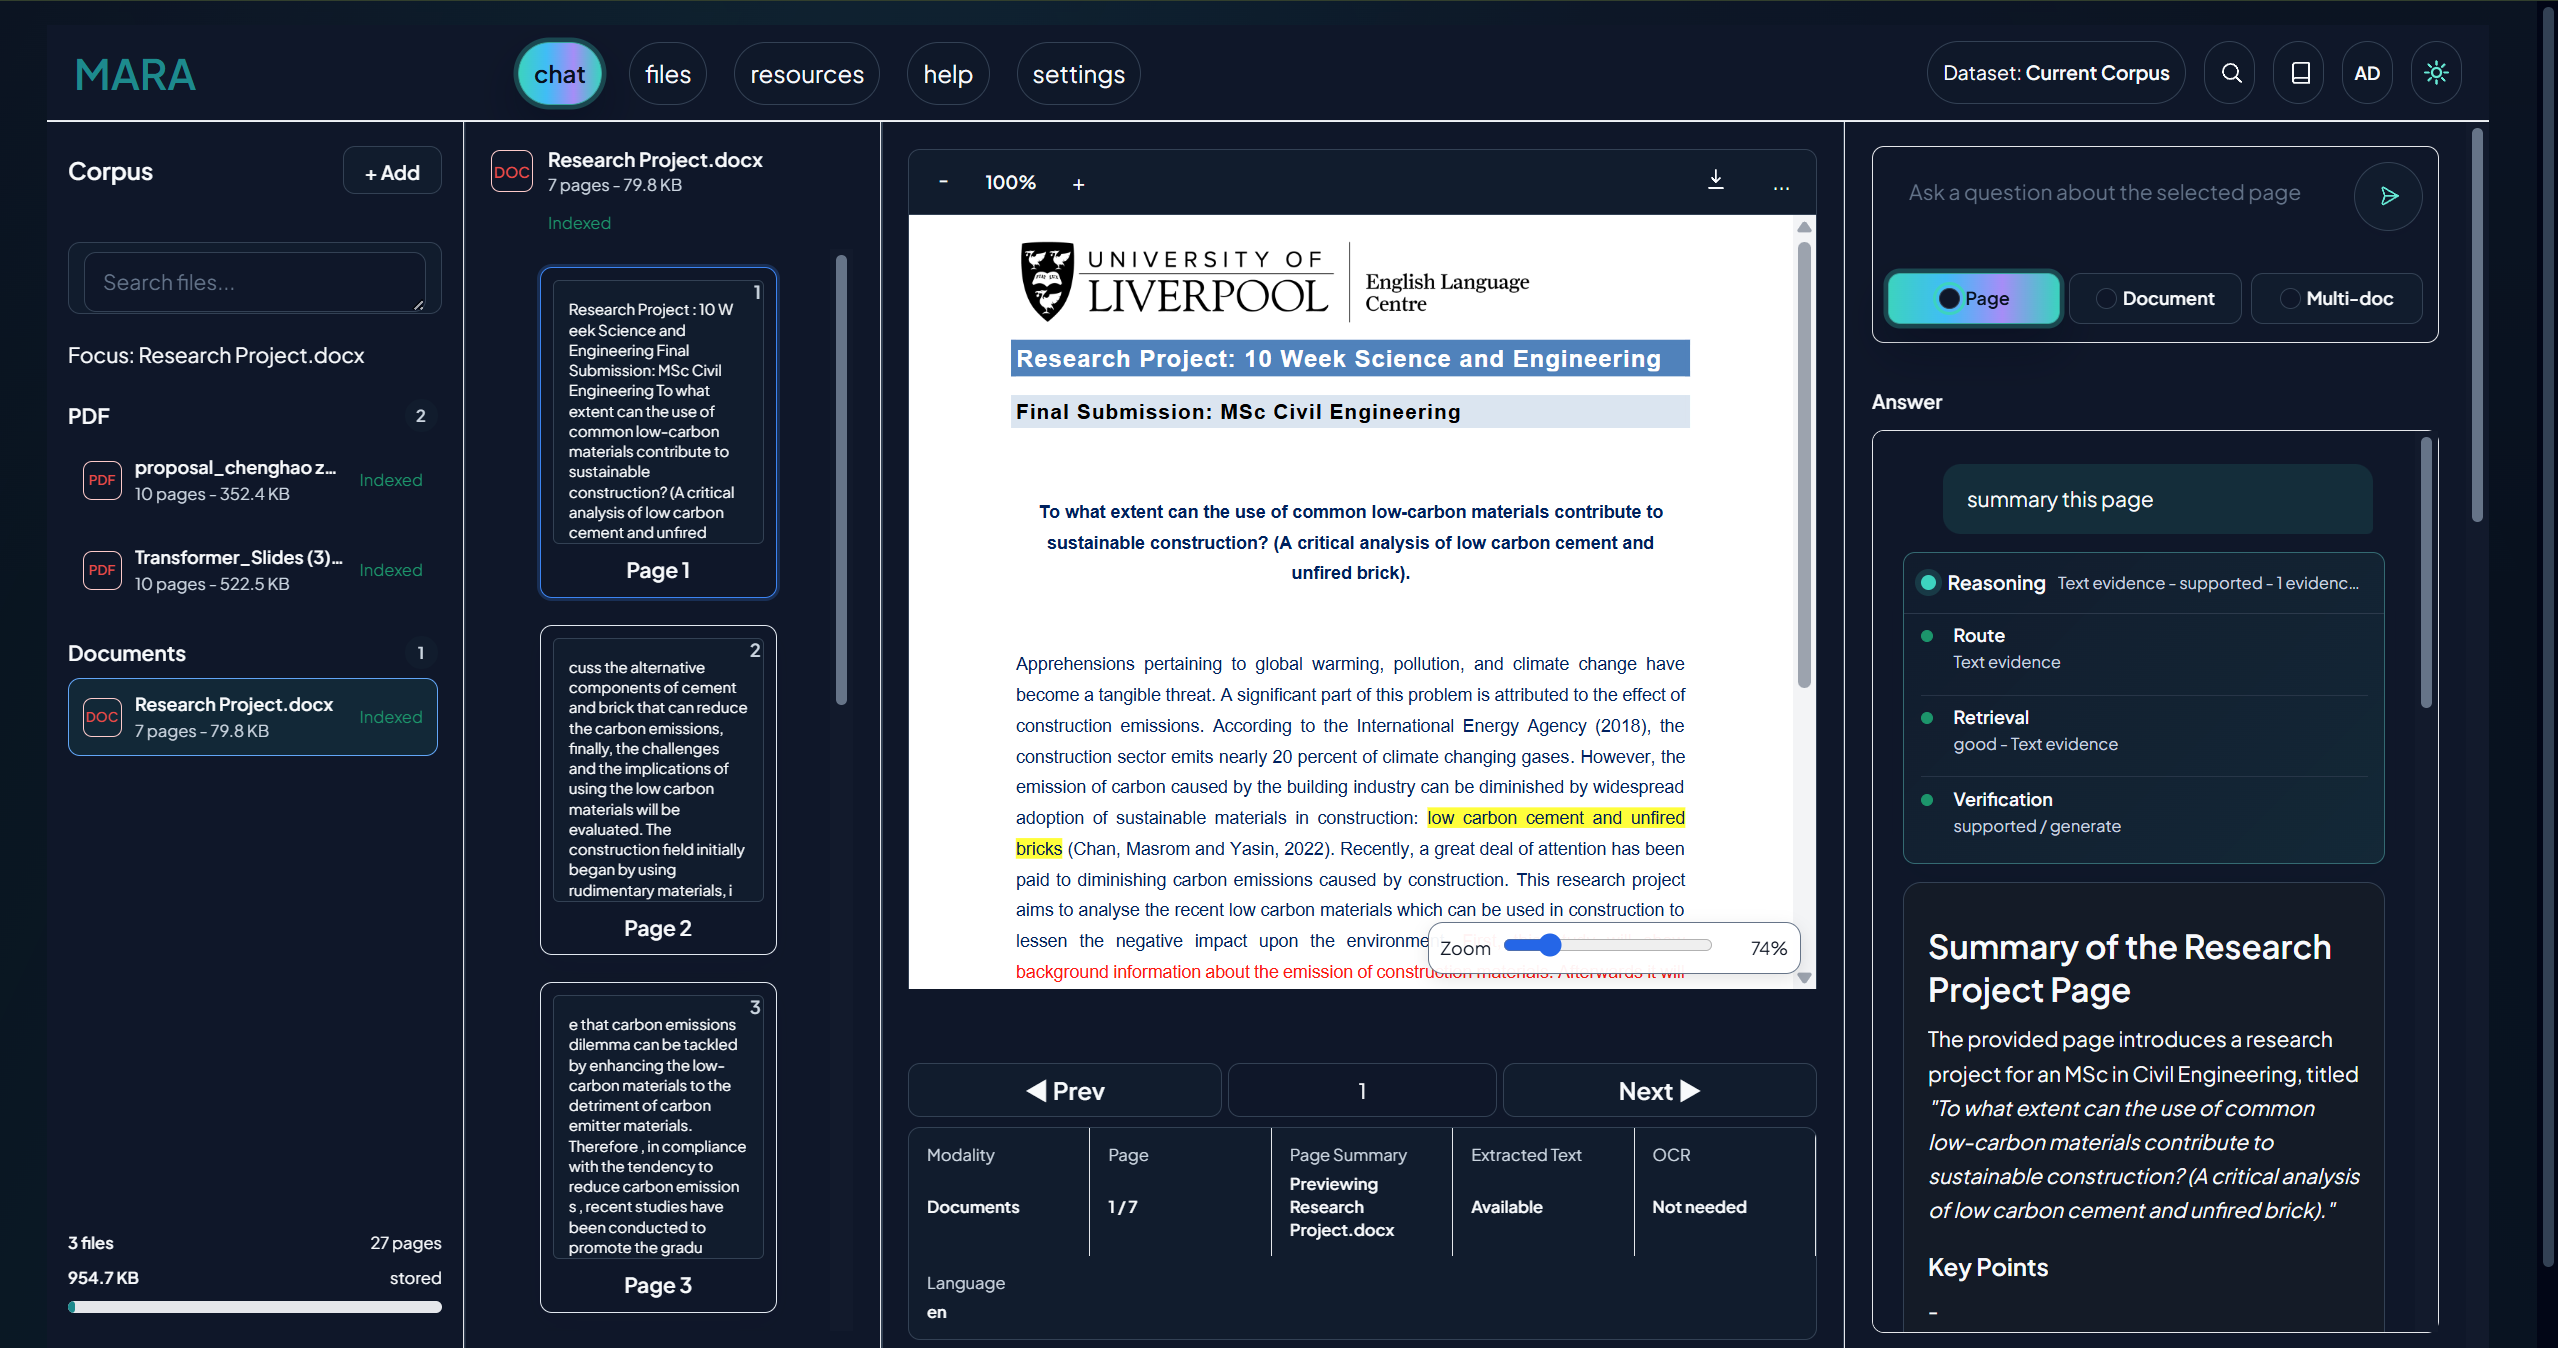
\includegraphics[width=\textwidth]{figures/mara-ui-qa.png}
\caption{Live MARA UI screenshot on the non-sensitive demonstration document \texttt{ResearchProject.docx}: source selection, page preview, routed answer, evidence metadata, retrieval status, and controller trace in one QA workflow.}
\label{fig:ui}
\end{figure*}

The CLI walkthrough supports the same scenario without a browser:
\begin{quote}\small
\texttt{MARA docqa index ./docs/report.pdf}\\
\texttt{MARA docqa files}\\
\texttt{MARA docqa ask -{}-file report.pdf -{}-reasoning mara -{}-prompt "..."}
\end{quote}
The benchmark walkthrough starts from route manifests and produces prediction records, route metrics, and synthesis tables. This is important for a demo paper: route-aware behaviour is not only visible in the UI, but also reproducible through a public release tag and supplementary benchmark bundle whose synthesis script, backend metadata, and evaluator status are recorded in the appendix.

The intended demonstration has three short scenarios. First, a UI scenario indexes \texttt{ResearchProject.docx} and asks a question whose answer requires source-grounded evidence. The demo highlights document selection, answer generation, citations, and the route trace. Second, a CLI scenario repeats a similar workflow without launching the browser, showing that \texttt{MARA docqa} is not a separate implementation but a reproducible surface over the same runtime. Third, a benchmark scenario opens the full-system synthesis tables and connects the UI-visible route trace to aggregate route metrics. The Codex and Claude Code wrappers are shown only as optional platform integrations, with details left to the appendix.

\ifmaravenue
\paragraph{Availability.}
\ifmaraanonymous
The anonymized submission package includes an installable MARA archive and the full-system benchmark synthesis bundle. A venue submission must pair this paper with a short supplementary demonstration video showing the Web UI QA loop, a browser-free CLI flow, and the benchmark artifact walkthrough. Public repository links are omitted from this anonymous version.
\else
The venue-facing demo package is anchored at the public MARA release \texttt{v0.0.40}\footnote{\url{https://github.com/262412/MARA/releases/tag/v0.0.40}}. The submission package includes the companion full-system benchmark synthesis bundle\footnote{\path{mara-full-system-benchmark-synthesis-v0.0.40.zip}}. A venue submission must pair this paper with a short supplementary demonstration video showing the Web UI QA loop, a browser-free CLI flow, and the benchmark artifact walkthrough.
\fi
\fi

\section{Related Work}

\subsection{Route-Aware RAG and Verification}

RAG systems retrieve external evidence before generation and are a standard pattern for knowledge-intensive QA \citep{lewis2020rag,karpukhin2020dpr,gao2023rag}. Their weakness is that retrieval is often treated as a fixed step. MARA instead treats route choice, evidence adequacy, and abstention as observable controller decisions.

Self-RAG motivates this design by learning when to retrieve and when to critique retrieved evidence \citep{asai2023selfrag}. MARA does not reproduce Self-RAG training. It uses the decision structure as a system-level controller. Adaptive RAG systems similarly motivate route selection by question type and difficulty \citep{jeong2024adaptiverag}. Corrective RAG (CRAG) highlights the need to judge retrieval quality before generation \citep{yan2024crag}; MARA includes guarded retrieval and verification states that can retry, switch, or abstain.

\subsection{Multimodal Document QA and Workbenches}

Multimodal document QA adds further route pressure. Page-image retrieval methods such as ColPali preserve layout and visual details that OCR chunks can lose \citep{faysse2024colpali}. MMDocRAG benchmarks retrieval-augmented multimodal generation for document QA and exposes text/visual trade-offs \citep{dong2025mmdocrag}. GraphRAG methods are useful for global summarisation and cross-document questions \citep{edge2024graphrag}, while datasets such as QASPER, ALCE, RAGTruth, and SlideVQA expose long-document evidence, citations, hallucination risk, and visual QA \citep{dasigi2021qasper,gao2023alce,niu2024ragtruth,tanaka2023slidevqa}.

MARA sits between these lines of work. It is a local workbench with practical UI and CLI affordances, but its main research-facing object is the controller trace: route, evidence, verification, cost, and abstention decisions that can be inspected by a user and measured by a benchmark harness.

\section{Conclusion}

MARA's strongest current result is not a single benchmark number. It is the integration of UI, CLI, controller trace, evidence records, and route-level evaluation into one local-first system. The controller makes routing inspectable: users can see not only an answer, but also the route, evidence, citations, verifier status, workflow cost, optional planner scoring fields, recovery routes, and abstention behaviour.

The limitations are important. The controller is rule-based by default: it combines heuristic planning with route-probe scoring when probes are available, but it is not a trained or calibrated router. Element and graph routes are implemented as prototype or scoped routes and need stronger evidence indexes and task-specific evaluation before they should be framed as mature. Page-image/VLM support depends on configured visual retrieval and generation backends, which can be slower than text routes and may run in evidence-only mode when the VLM backend is unavailable. The full-system benchmark did not use paper-grade external evaluators; it reports local dataset-native and MARA diagnostic metrics. A later RAGTruth prompt-budget repair was a post-hoc targeted diagnostic. It verified that the prompt-length failure mode had been repaired on a small subset, but it is not mixed into the main benchmark table because it was not run under the same full-system protocol.

These constraints shape the next steps: expand full-protocol reruns only after concrete system changes, improve element and graph evidence quality, and replace rule-based routing with a trained or calibrated router only after enough controller traces are available. Even in its current form, MARA demonstrates that a local document QA workbench can make retrieval, routing, evidence, and abstention visible to both users and evaluators.
